\documentclass[tikz,border=7pt]{standalone}
\usepackage[T1]{fontenc}
\usepackage{lmodern}
\usetikzlibrary{arrows.meta,positioning,shapes.geometric,fit,backgrounds,calc}
\begin{document}
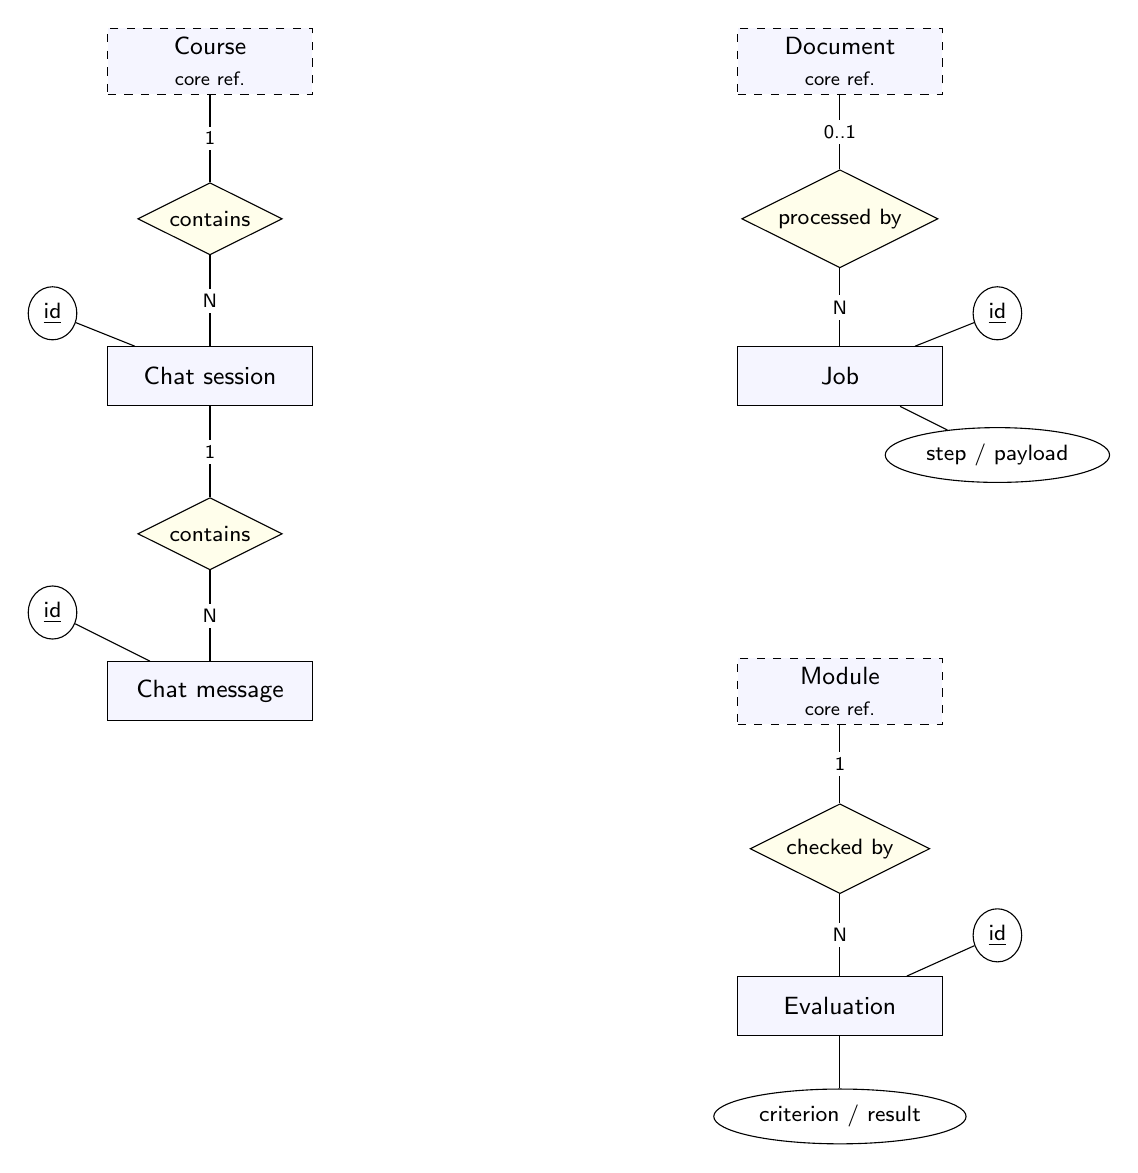
\begin{tikzpicture}[font=\sffamily\small,>=Latex,
box/.style={draw,rounded corners=2pt,align=center,minimum width=3cm,minimum height=1cm,fill=blue!4},
entity/.style={draw,rectangle,align=center,minimum width=2.6cm,minimum height=.75cm,fill=blue!4},
rel/.style={draw,diamond,aspect=2,inner sep=2pt,align=center,font=\sffamily\footnotesize,fill=yellow!8},
attr/.style={draw,ellipse,inner sep=3pt,font=\sffamily\footnotesize},
uc/.style={draw,ellipse,align=center,minimum width=4cm,minimum height=.9cm},
flow/.style={->,thick},lab/.style={font=\sffamily\scriptsize,fill=white,inner sep=2pt}]
\node[entity,dashed] (c) at (0,6) {Course\\{\scriptsize core ref.}};
\node[entity,dashed] (d) at (8,6) {Document\\{\scriptsize core ref.}};
\node[entity] (j) at (8,2) {Job};
\node[entity] (se) at (0,2) {Chat session};
\node[entity] (msg) at (0,-2) {Chat message};
\node[entity,dashed] (m) at (8,-2) {Module\\{\scriptsize core ref.}};
\node[entity] (ev) at (8,-6) {Evaluation};
\node[rel] (sessions) at (0,4) {contains}; \draw (c) -- node[lab]{1} (sessions); \draw (sessions) -- node[lab]{N} (se);
\node[rel] (msgs) at (0,0) {contains}; \draw (se) -- node[lab]{1} (msgs); \draw (msgs) -- node[lab]{N} (msg);
\node[rel] (jobs) at (8,4) {processed by}; \draw (d) -- node[lab]{0..1} (jobs); \draw (jobs) -- node[lab]{N} (j);
\node[rel] (checks) at (8,-4) {checked by}; \draw (m) -- node[lab]{1} (checks); \draw (checks) -- node[lab]{N} (ev);
\node[attr] (jid) at (10,2.8) {\underline{id}}; \draw (j) -- (jid);
\node[attr] (step) at (10,1) {step / payload}; \draw (j) -- (step);
\node[attr] (seid) at (-2,2.8) {\underline{id}}; \draw (se) -- (seid);
\node[attr] (msgid) at (-2,-1) {\underline{id}}; \draw (msg) -- (msgid);
\node[attr] (evid) at (10,-5.1) {\underline{id}}; \draw (ev) -- (evid);
\node[attr] (criterion) at (8,-7.4) {criterion / result}; \draw (ev) -- (criterion);
\end{tikzpicture}
\end{document}
